\documentclass[letter,11pt]{article}

\usepackage[spanish,es-nodecimaldot]{babel}
\usepackage[utf8]{inputenc}

\usepackage{lmodern}
\usepackage[T1]{fontenc}
\usepackage{textcomp}

\usepackage{framed}
\usepackage[svgnames]{xcolor}
\colorlet{shadecolor}{Gainsboro!50}

\usepackage[labelfont=bf]{caption}
\usepackage{graphicx}
\usepackage{pstricks}

\usepackage{anysize}
\marginsize{3cm}{2cm}{2cm}{3cm}

\usepackage{siunitx}
\usepackage{amsmath}
\usepackage{array}
\usepackage{csquotes}
\usepackage{steinmetz}
\usepackage{stmaryrd}

\usepackage{fancyhdr}
\usepackage{lastpage}
\pagestyle{fancy}
\fancyhf{}
\fancyhead[LE,RO]{Laboratorio de Circuitos Eléctricos III}
\fancyfoot[CO,CE]{\thepage\ de \pageref{LastPage}}

\special{papersize=215.9mm,279.4mm}

\usepackage[
    pdfauthor={Carlos Eduardo Caballero Burgoa},%
    pdftitle={Laboratorio de Circuitos Eléctricos III},%
    pdfsubject={Medida de la potencia activa y reactiva trifásica en circuitos
    con carga equilibrada},%
    colorlinks,%
    citecolor=black,%
    filecolor=black,%
    linkcolor=black,%
    urlcolor=black,
    breaklinks]{hyperref}
\usepackage{breakurl}

\renewcommand{\arraystretch}{1.2}

\begin{document}

\begin{titlepage}
    \begin{center}
        {\Large UNIVERSIDAD MAYOR DE SAN SIMÓN}\\
        \vspace*{0.15cm}
        {\large FACULTAD DE CIENCIAS Y TECNOLOGÍA}\\
        \vspace*{0.10cm}
        DEPARTAMENTO DE ELÉCTRICA-ELECTRÓNICA\\
        \vspace*{3.0cm}
        {\Large \textbf{LABORATORIO DE CIRCUITOS ELÉCTRICOS III}}\\
        \vspace*{0.3cm}
        {\Large \textbf{INFORME No. 5}}\\
        \vspace*{3.5cm}
        {\Large \textbf{MEDIDA DE LA POTENCIA ACTIVA Y REACTIVA\\
        TRIFÁSICA EN CIRCUITOS CON CARGA EQUILIBRADA}}\\
    \end{center}

    \vspace*{5.8cm}
    \leftskip=7.95cm
    \noindent
    \textbf{Estudiante:}\\
    Caballero Burgoa, Carlos Eduardo.\\
    \newline
    \textbf{Carrera:}\\
    Ing. Electromecánica.\\
    \newline
    \textbf{Docente:}\\
    Ing. Marco Antonio Vallejo Camacho.\\
    \newline
    \textbf{Grupo:} 2F (Martes).\\
\textbf{Fecha de entrega:} 23 de Octubre del 2024.\\
\end{titlepage}

\section{Cálculos teóricos}

\subsection{Carga en estrella}
Considerando un circuito trifásico delta-estrella equilibrado
(\textbf{Figura~\ref{circuito1}}):

Con voltajes de linea $U_L=220[\text{V}]$ y con frecuencia de $50[\text{Hz}]$,
se hallan las potencias activa y reactiva:

\begin{figure}[!h]
\centering
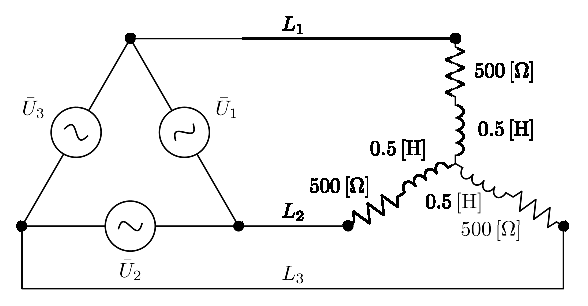
\includegraphics[scale=0.95]{figura1.eps}
\caption{Circuito trifásico equilibrado delta-estrella.}
\label{circuito1}
\end{figure}

Se calcula la frecuencia angular ($\omega$):
\begin{equation*}
    \begin{split}
        \omega &= 2\pi f\\
               &= 2\pi(50)\\
               &= 100\pi[\text{rad}/\text{s}]\\
    \end{split}
\end{equation*}

Se halla la impedancia en el dominio de frecuencia:
\begin{equation*}
    \begin{split}
        Z &= R_2+j\omega L\\
          &= 500+j50\pi[\Omega]\\
    \end{split}
\end{equation*}

Y su representación fasorial:
\begin{equation*}
    \begin{split}
        |Z| &= \sqrt{500^2+(50\pi)^2}\\
            &= 524.09\\
        \theta &= \arctan\left(\frac{50\pi}{500}\right)\\
               &= 17.44^{\circ}\\
        Z &= 524.09\phase{17.44^{\circ}}[\Omega]\\
    \end{split}
\end{equation*}

A partir del voltaje de linea, se calcula el voltaje de fase:
\begin{equation*}
    \begin{split}
        U_F &= \frac{U_L}{\sqrt{3}}\\
            &= \frac{220}{\sqrt{3}}\\
            &= 127.02[\text{V}]\\
    \end{split}
\end{equation*}

Y a partir del voltaje de fase, se halla la corriente de linea:
\begin{equation*}
    \begin{split}
        I_L &= \frac{U_F}{|Z|}\\
            &= \frac{127.02}{\sqrt{(500)^2+(50\pi)^2}}\\
            &= 0.24[\text{A}]\\
    \end{split}
\end{equation*}

Por tanto las potencias activa y reactiva son:
\begin{equation*}
    \begin{split}
        P_T &= \sqrt{3}\,U_L\,I_L\,\cos(\phi)\\
            &= 220\,0.24\,\cos(17.44^{\circ})\\
            &= 88.104[\text{W}]\\
        Q_T &= \sqrt{3}\,U_L\,I_L\,\sen(\phi)\\
            &= 220\,0.24\,\sen(17.44^{\circ})\\
            &= 27.679[\text{VAR}]\\
    \end{split}
\end{equation*}

\subsection{Carga en delta}
Considerando un circuito trifásico delta-delta equilibrado
(\textbf{Figura~\ref{circuito2}}):

Con voltajes de linea $U_L=220[\text{V}]$ y con frecuencia de $50[\text{Hz}]$,
se hallan las potencias activa y reactiva:

\begin{figure}[!h]
\centering
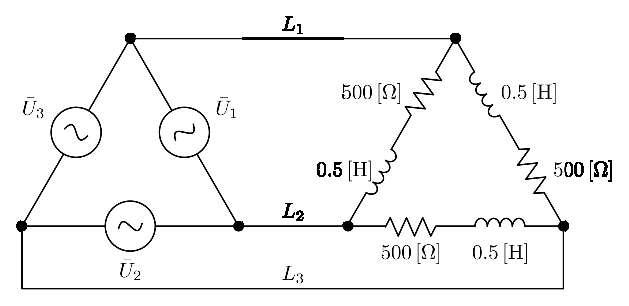
\includegraphics[scale=0.95]{figura2.eps}
\caption{Circuito trifásico equilibrado delta-delta.}
\label{circuito2}
\end{figure}

A partir del voltaje de linea, se calcula la corriente de fase:
\begin{equation*}
    \begin{split}
        I_F &= \frac{U_L}{|Z|}\\
            &= \frac{220}{\sqrt{(500)^2+(50\pi)^2}}\\
            &= 0.4198[\text{A}]\\
    \end{split}
\end{equation*}

Y a partir de la corriente de linea se obtiene la corriente de fase:
\begin{equation*}
    \begin{split}
        I_L &= \sqrt{3}\,I_F\\
            &= \sqrt{3}\,(0.4198)\\
            &= 0.7271[\text{A}]\\
    \end{split}
\end{equation*}

Por tanto las potencias activa y reactiva son:
\begin{equation*}
    \begin{split}
        P_T &= \sqrt{3}\,U_L\,I_L\,\cos(\phi)\\
            &= 220\,0.7271\,\cos(17.44^{\circ})\\
            &= 264.31[\text{W}]\\
        Q_T &= \sqrt{3}\,U_L\,I_L\,\sen(\phi)\\
            &= 220\,0.7271\,\sen(17.44^{\circ})\\
            &= 83.036[\text{VAR}]\\
    \end{split}
\end{equation*}

\subsection{Resumen de resultados}
En la siguiente tabla se resumen los valores obtenidos teóricamente:

\begin{center}
    \begin{tabular}{|c||c|c|}
    \hline
    & \textbf{Carga Estrella} & \textbf{Carga Delta}
    \tabularnewline \hline \hline
    $P_T$ &
    $88.104[\text{W}]$ &
    $264.31[\text{W}]$
    \tabularnewline \hline
    $Q_T$ &
    $27.679[\text{VAR}]$ &
    $83.036[\text{VAR}]$
    \tabularnewline \hline
    \end{tabular}
\end{center}

\section{Simulación}
Se utilizó el software \emph{Electronic Workbench v5.12.} para simular
los circuitos calculados, la carga en estrella puede verse en la
\textbf{Figura~\ref{simulacion1}}, mientras que la carga en delta puede verse en
la \textbf{Figura~\ref{simulacion2}}:

\begin{figure}[!h]
\centering
\includegraphics[scale=1.00]{simulacion/practica5.1.eps}
\caption{Simulación del circuito delta-estrella.}
\label{simulacion1}
\end{figure}

\begin{figure}[!h]
\centering
\includegraphics[scale=1.00]{simulacion/practica5.2.eps}
\caption{Simulación del circuito delta-estrella.}
\label{simulacion2}
\end{figure}

\subsection{Resumen de resultados}
En la siguiente tabla se resumen los valores obtenidos de la simulación: 

\begin{center}
    \begin{tabular}{|c||c|c|c||c|c|c|}
    \hline
    & \multicolumn{3}{|c||}{\textbf{Carga Estrella}} &
    \multicolumn{3}{|c|}{\textbf{Carga Delta}}
    \tabularnewline \hline \hline
    & $Z_1$ & $Z_2$ & $Z_3$ & $Z_1$ & $Z_2$ & $Z_3$
    \tabularnewline \hline \hline
    $I_Z$ &
    $242.1[m\text{A}]$ & $242.0[m\text{A}]$ & $242.0[m\text{A}]$ &
    $418.6[m\text{A}]$ & $418.6[m\text{A}]$ & $418.6[m\text{A}]$
    \tabularnewline \hline
    $U_R$ &
    $121.0[\text{V}]$ & $120.9[\text{V}]$ & $120.9[\text{V}]$ &
    $209.3[\text{V}]$ & $209.2[\text{V}]$ & $209.3[\text{V}]$
    \tabularnewline \hline
    $U_X$ &
    $38.51[\text{V}]$ & $38.52[\text{V}]$ & $38.52[\text{V}]$ &
    $66.59[\text{V}]$ & $66.64[\text{V}]$ & $66.59[\text{V}]$
    \tabularnewline \hline \hline
    $P=U_R\,I_Z$ &
    $29.29[\text{W}]$ & $29.26[\text{W}]$ & $29.26[\text{W}]$ &
    $87.61[\text{W}]$ & $87.57[\text{W}]$ & $87.61[\text{W}]$
    \tabularnewline \hline
    $Q=U_X\,I_Z$ &
    $9.32[\text{VAR}]$ & $9.32[\text{VAR}]$ & $9.32[\text{VAR}]$ &
    $27.87[\text{VAR}]$ & $27.90[\text{VAR}]$ & $27.87[\text{VAR}]$
    \tabularnewline \hline \hline
    $P_T$ &
    \multicolumn{3}{|c||}{$87.81[\text{W}]$} &
    \multicolumn{3}{|c|}{$262.80[\text{W}]$}
    \tabularnewline \hline
    $Q_T$ &
    \multicolumn{3}{|c||}{$27.967[\text{VAR}]$} &
    \multicolumn{3}{|c|}{$83.645[\text{VAR}]$}
    \tabularnewline \hline
    \end{tabular}
\end{center}

\section{Tablas y mediciones}
Se presentan los resultados obtenidos con las mediciones realizadas en 
laboratorio y el calculo de la potencia a partir del voltaje y corriente:

\begin{center}
    \begin{tabular}{|c||c|c|c||c|c|c|}
    \hline
    & \multicolumn{3}{|c||}{\textbf{Carga Estrella}} &
    \multicolumn{3}{|c|}{\textbf{Carga Delta}}
    \tabularnewline \hline \hline
    & $Z_1$ & $Z_2$ & $Z_3$ & $Z_1$ & $Z_2$ & $Z_3$
    \tabularnewline \hline \hline
    $I_Z[\text{A}]$ & $0.22$ & $0.23$ & $0.23$ & $0.40$ & $0.41$ & $0.40$
    \tabularnewline \hline
    $U_R[\text{V}]$ & $124$ & $125$ & $125$ & $217$ & $217$ & $215$
    \tabularnewline \hline
    $U_X[\text{V}]$ & $37.6$ & $37.9$ & $37.5$ & $66.4$ & $66.9$ & $65.4$
    \tabularnewline \hline \hline
    $P=U_R\,I_Z[\text{W}]$ &
    $27.28$ & $28.75$ & $28.75$ & $86.80$ & $88.97$ & $86.00$
    \tabularnewline \hline
    $Q=U_X\,I_Z[\text{VAR}]$ &
    $8.272$ & $ 8.717$ & $ 8.625$ & $26.56$ & $27.429$ & $26.16$
    \tabularnewline \hline \hline
    $P_T$ &
    \multicolumn{3}{|c||}{$84.78[\text{W}]$} &
    \multicolumn{3}{|c|}{$261.77[\text{W}]$}
    \tabularnewline \hline
    $Q_T$ &
    \multicolumn{3}{|c||}{$25.614[\text{VAR}]$} &
    \multicolumn{3}{|c|}{$80.149[\text{VAR}]$}
    \tabularnewline \hline
    \end{tabular}
\end{center}

Se presentan los resultados obtenidos con las mediciones realizadas con el
método de los dos vatímetros para el calculo de potencia:

\begin{center}
    \begin{tabular}{|c||c|c|}
    \hline
    & \textbf{Carga Estrella} & \textbf{Carga Delta}
    \tabularnewline \hline \hline
    $W_1$ & $39[\text{W}]$ & $115[\text{W}]$
    \tabularnewline \hline
    $W_2$ & $55[\text{W}]$ & $162[\text{W}]$
    \tabularnewline \hline
    $Q_1$ & $39[\text{VAR}]$ & $122[\text{VAR}]$
    \tabularnewline \hline
    $Q_2$ & $-7[\text{VAR}]$ & $-40[\text{VAR}]$
    \tabularnewline \hline \hline
    $P_T$ & $94[\text{W}]$ & $277[\text{W}]$
    \tabularnewline \hline
    $Q_T$ & $32[\text{VAR}]$ & $82[\text{VAR}]$
    \tabularnewline \hline
    \end{tabular}
\end{center}

\subsection{Resumen de resultados}
En la siguiente tabla se resumen los valores obtenidos del calculo teórico,
la simulación y los datos obtenidos de laboratorio:

\begin{center}
    \begin{tabular}{|c||c|c|c|c|}
    \hline
    & \multicolumn{2}{|c|}{\textbf{Carga Estrella}} &
    \multicolumn{2}{|c|}{\textbf{Carga Delta}}
    \tabularnewline \hline
    & $P_T[\text{W}]$ & $Q_T[\text{VAR}]$ &
    $P_T[\text{W}]$ & $Q_T[\text{VAR}]$
    \tabularnewline \hline \hline
    \textbf{Teórico} &
    $88.104$ & $27.679$ &
    $264.31$ & $83.036$
    \tabularnewline \hline
    \textbf{Simulado} &
    $ 87.81$ & $27.967$ &
    $262.80$ & $83.645$
    \tabularnewline \hline
    \textbf{Laboratorio ($U{\times}I$)} &
    $ 84.78$ & $25.614$ &
    $261.77$ & $80.149$
    \tabularnewline \hline
    \textbf{Laboratorio (Dos vatímetros)} &
    $94$ & $32$ &
    $277$ & $82$
    \tabularnewline \hline
    \end{tabular}
\end{center}

\section{Cuestionario}

\begin{enumerate}

\item \textbf{Compare las potencias activa y reactiva trifásica obtenidas con
carga en delta y carga en estrella, ¿Cual es la relación en ambos casos? ¿Dicha
relación se verifica con lo aprendido teóricamente?}

Las potencias activa y reactiva calculadas, y la relación entre una carga
estrella y delta son:

\begin{center}
    \begin{tabular}{|c|c||c|c||c|}
    \hline
    \multicolumn{2}{|c||}{} & $\text{Y}$ & $\triangle$ & Relación $\triangle/Y$
    \tabularnewline \hline \hline
    \textbf{Teórico} & \textbf{Activa} &
    $88.104$ & $264.31$ & $2.9999$
    \tabularnewline \hline
    & \textbf{Reactiva} &
    $27.679$ & $83.036$ & $2.9999$
    \tabularnewline \hline \hline
    \textbf{Simulado} & \textbf{Activa} &
    $87.81$ & $262.80$ & $2.9928$
    \tabularnewline \hline
    & \textbf{Reactiva} &
    $27.967$ & $83.645$ & $2.9908$
    \tabularnewline \hline \hline
    \textbf{Laboratorio ($U{\times}I$)} & \textbf{Activa} &
    $84.78$ & $261.77$ & $3.0876$
    \tabularnewline \hline
    & \textbf{Reactiva} &
    $25.614$ & $80.149$ & $3.1291$
    \tabularnewline \hline \hline
    \textbf{Laboratorio (Dos vatímetros)} & \textbf{Activa} &
    $94$ & $227$ & $2.4149$
    \tabularnewline \hline
    & \textbf{Reactiva} &
    $32$ & $82$ & $2.5625$
    \tabularnewline \hline
    \end{tabular}
\end{center}

La relación teórica $P_\triangle = 3\,P_{\text{Y}}$ se verifica en todos los
casos con margenes aceptables de error.

\item \textbf{La potencia medida en cada impedancia, ¿es la misma o no?. En caso
de que sea diferente explique las posibles razones.}

Las potencias obtenidas en cada impedancia son las siguientes:

\begin{center}
    \begin{tabular}{|c||c|c|c||c|c|c|}
    \hline
    & \multicolumn{3}{|c||}{\textbf{Carga Estrella}} &
    \multicolumn{3}{|c|}{\textbf{Carga Delta}}
    \tabularnewline \hline \hline
    $P[\text{W}]$ &
    $27.28$ & $28.75$ & $28.75$ & $86.80$ & $88.97$ & $86.00$
    \tabularnewline \hline
    $Q[\text{VAR}]$ &
    $8.272$ & $ 8.717$ & $ 8.625$ & $26.56$ & $27.429$ & $26.16$
    \tabularnewline \hline
    \end{tabular}
\end{center}

Las variaciones son despreciables, y pueden deberse a los valores de las
resistencias e inductores, a los conectores, a los instrumentos medición o
a los voltajes de linea usados, que pueden generar pequeños desequilibrios en
el circuito.

\item \textbf{Comparar la potencia total obtenida por los dos métodos. ¿Existe
diferencia en dichos valores? ¿En que caso se obtiene un valor mas cercano al
teórico y por que?}

Los valores comparados de la potencia son:

\begin{center}
    \begin{tabular}{|c|c||c||c|c||c|}
    \hline
    \multicolumn{2}{|c||}{} &
    \textbf{Teórico} & $U{\times}I$ & \textbf{Dos vatímetros} & \textbf{Error}
    \tabularnewline \hline \hline
    \textbf{Carga Estrella} & $P_T$ &
    $88.104[\text{W}]$ & $84.78[\text{W}]$ & $94[\text{W}]$ & $9.81\%$
    \tabularnewline \hline
                   & $Q_T$ &
    $27.679[\text{VAR}]$ & $25.614[\text{VAR}]$ & $32[\text{VAR}]$ & $19.96\%$
    \tabularnewline \hline \hline
    \textbf{Carga Delta} & $P_T$ &
    $246.31[\text{W}]$ & $261.77[\text{W}]$ & $277[\text{W}]$ & $5.5\%$
    \tabularnewline \hline
                & $Q_T$ &
    $83.036[\text{VAR}]$ & $80.149[\text{VAR}]$ & $82[\text{VAR}]$ & $2.26\%$
    \tabularnewline \hline
    \end{tabular}
\end{center}

Existen diferencias pequeñas entre los valores obtenidos, los valores más
cercanos a los valores teóricos son: los calculados a partir del producto del
voltaje y corriente, esto puede deberse a la escala en la que trabaja el
vatímetro utilizado.

\item \textbf{Demuestre que la potencia total en un circuito trifásico
equilibrado independientemente de la forma de conexión de la carga esta dada
por: $P_T = \sqrt{3}\,U_L\,I_L\,\cos(\phi)$ y a partir de esto, verifique la
relación entre un sistema delta y estrella: $P_{\triangle} = 3\,P_{\text{Y}}$}.

En un elemento de la carga, la tensión y corriente de fase son:
\begin{equation*}
    \begin{split}
        v_a(t) &= \sqrt{2}\,v_{\text{rms}}\,\cos(\omega{t})\\
        i_a(t) &= \sqrt{2}\,i_{\text{rms}}\,\cos(\omega{t} - \phi)\\
    \end{split}
\end{equation*}


La potencia instantánea por fase esta dada por la siguiente expresión:
\begin{equation*}
    \begin{split}
        p_a(t) &= v_a(t)\,i_a(t)\\
               &= \sqrt{2}\,U_f\,\cos(\omega{t})
                  \sqrt{2}\,I_f\,\cos(\omega{t}-\phi)\\
               &= 2\,U_f\,I_f\,\cos(\omega{t})\cos(\omega{t}-\phi)\\
        p_b(t) &= 2\,U_f\,I_f\,\cos(\omega{t}-120^{\circ})\cos(\omega{t}-\phi-120^{\circ})\\
        p_c(t) &= 2\,U_f\,I_f\,\cos(\omega{t}+120^{\circ})\cos(\omega{t}-\phi+120^{\circ})\\
    \end{split}
\end{equation*}

La potencia total es la suma de las potencias en las tres fases:
\begin{equation*}
    \begin{split}
        p(t) =\,& p_a(t)+p_b(t)+p_c(t)\\
             =\,& 2\,U_f\,I_f\,\cos(\omega{t})\cos(\omega{t}-\phi)+\\
                & 2\,U_f\,I_f\,\cos(\omega{t}-120^{\circ})\cos(\omega{t}-\phi-120^{\circ})+\\
                & 2\,U_f\,I_f\,\cos(\omega{t}+120^{\circ})\cos(\omega{t}-\phi+120^{\circ})\\
    \end{split}
\end{equation*}

Considerando la siguiente identidad trigonométrica:
\begin{equation*}
    \cos(A)\,\cos(B) = \frac{1}{2}\left[\cos(A+B)+\cos(A-B)\right]
\end{equation*}

Se obtiene la siguiente expresión:
\begin{equation*}
    \begin{split}
        p(t) =\,& 2\,U_f\,I_f(
                  \cos(\omega{t})\cos(\omega{t}-\phi)+\\
                & \cos(\omega{t}-120^{\circ})\cos(\omega{t}-\phi-120^{\circ})+
                  \cos(\omega{t}+120^{\circ})\cos(\omega{t}-\phi+120^{\circ}))\\
             =\,& 2\,U_f\,I_f(\\
                & \frac{1}{2}\left[\cos(2\omega{t}-\phi)+\cos(\phi)\right]+\\
                & \frac{1}{2}\left[\cos(2\omega{t}-\phi-240^{\circ})+\cos(\phi)\right]+
                  \frac{1}{2}\left[\cos(2\omega{t}-\phi+240^{\circ})+\cos(\phi)\right])\\
             =\,& U_f\,I_f(
                  \cos(2\omega{t}-\phi)+\cos(\phi)+\\
                & \cos(2\omega{t}-\phi-240^{\circ})+\cos(\phi)+
                  \cos(2\omega{t}-\phi+240^{\circ})+\cos(\phi))\\
             =\,& U_f\,I_f(
                  3\cos(\phi)+\\
                & \cos(2\omega{t}-\phi)+
                  \cos(2\omega{t}-\phi-240^{\circ})+
                  \cos(2\omega{t}-\phi+240^{\circ}))\\
    \end{split}
\end{equation*}

Definiendo $\delta = 2\omega{t} - \phi$, se obtiene:
\begin{equation*}
    \begin{split}
        p(t) =\,& U_f\,I_f(
                  3\cos(\phi)+
                  \cos(\delta)+
                  \cos(\delta-240^{\circ})+
                  \cos(\delta+240^{\circ}))\\
    \end{split}
\end{equation*}

Considerando la siguiente identidad trigonométrica:
\begin{equation*}
    \cos(A{\pm}B) = \cos(A)\cos(B) \mp \sen(A)\sen(B)
\end{equation*}

Se obtiene la siguiente expresión:
\begin{equation*}
    \begin{split}
        p(t) =\,& U_f\,I_f(
                  3\cos(\phi)+
                  \cos(\delta)+\\
                & \cos(\delta)\cos(240^{\circ})+\sen(\delta)\sen(240^{\circ})+\\
                & \cos(\delta)\cos(240^{\circ})-\sen(\delta)\sen(240^{\circ}))\\
             =\,& U_f\,I_f(
                  3\cos(\phi)+
                  \cos(\delta)+\\
                & \cos(\delta)\cos(240^{\circ})-\sen(\delta)\sen(240^{\circ})+\\
                & \cos(\delta)\cos(240^{\circ})+\sen(\delta)\sen(240^{\circ}))\\
             =\,& U_f\,I_f(
                  3\cos(\phi)+
                  \cos(\delta)+
                  2\cos(\delta)\cos(240^{\circ}))\\
             =\,& U_f\,I_f(
                  3\cos(\phi)+
                  \cos(\delta)+
                  2\left(-\frac{1}{2}\right)\cos(\delta))\\
             =\,& 3\,U_f\,I_f\,\cos(\phi)\\
    \end{split}
\end{equation*}

Considerando la relación entre lineas y fases siguiente:

En una carga conectada en estrella:
\begin{equation*}
    \begin{split}
        U_L = \sqrt{3}\,U_f\\
        I_L = I_f\\
    \end{split}
\end{equation*}

En una carga conectada en delta:
\begin{equation*}
    \begin{split}
        U_L = U_f\\
        I_L = \sqrt{3}\,I_f\\
    \end{split}
\end{equation*}

La potencia total en función de sus valores de linea es:
\begin{equation*}
    p(t) = \sqrt{3}\,U_L\,I_L\,\cos(\phi)
\end{equation*}

Si se comparan las potencias según el tipo de carga, se tiene:

En una carga conectada en estrella:
\begin{equation*}
    \begin{split}
        I_L =\,& \frac{U_f}{|Z|}
            =\,  \frac{U_L}{\sqrt{3}|Z|}\\
        P_{\text{Y}} =\,& \sqrt{3}\,U_L\,I_L\,\cos(\phi)
                     =\,  \sqrt{3}\,U_L\,\frac{U_L}{\sqrt{3}|Z|}\,\cos(\phi)
                     =\,  \frac{U_L^2}{|Z|}\,cos(\phi)\\
    \end{split}
\end{equation*}

En una carga conectada en delta:
\begin{equation*}
    \begin{split}
        I_f =\,& \frac{U_L}{|Z|}\\
        I_L =\,& \sqrt{3}\,I_f
            =\,  \frac{\sqrt{3}\,U_L}{|Z|}\\
        P_{\triangle} =\,& \sqrt{3}\,U_L\,I_L\,\cos(\phi)
                      =\,  \sqrt{3}\,U_L\,\frac{\sqrt{3}\,U_L}{|Z|}\,\cos(\phi)
                      =\,  3\frac{U_L^2}{|Z|}\,cos(\phi)\\
    \end{split}
\end{equation*}

Por tanto:
\begin{equation*}
    P_{\triangle} = 3\,P_{\text{Y}}
\end{equation*}

\item \textbf{Demuestre que el método de los dos vatímetros nos da la potencia
trifásica total en un circuito equilibrado.}

La potencia en los vatímetros será:
\begin{equation*}
    \begin{split}
        P_{W_1} =\,& \Re\{U_{AB}\,I^{*}_A\}\\
                =\,& U_L\,I_L\,\cos(\theta + 30^{\circ})\\
        P_{W_2} =\,& \Re\{U_{CB}\,I^{*}_C\}\\
                =\,& U_L\,I_L\,\cos(\theta - 30^{\circ})\\
    \end{split}
\end{equation*}

Considerando la siguiente identidad trigonométrica:
\begin{equation*}
    \cos(A{\pm}B) = \cos(A)\cos(B) \mp \sen(A)\sen(B)
\end{equation*}

La potencia total es:
\begin{equation*}
    \begin{split}
        P =\,& P_{W_1} + P_{W_2}\\
          =\,& U_L\,I_L\,\cos(\theta + 30^{\circ})+
               U_L\,I_L\,\cos(\theta - 30^{\circ})\\
          =\,& U_L\,I_L[\\
             & \cos(\theta)\,\cos(30^{\circ})-\sen(\theta)\,\sen(30^{\circ})+\\
             & \cos(\theta)\,\cos(30^{\circ})+\sen(\theta)\,\sen(30^{\circ})]\\
          =\,& U_L\,I_L[2\,\cos(\theta)\,\cos(30^{\circ})]\\
          =\,& U_L\,I_L\left[2\,\cos(\theta)\,\frac{\sqrt{3}}{2}\right]\\
          =\,& \sqrt{3}\,U_L\,I_L\,\cos(\theta)\\
    \end{split}
\end{equation*}

La suma de las lecturas de los vatímetros da por resultado la potencia promedio
total.

\end{enumerate}

\section{Conclusiones y Recomendaciones}
Se calcularon, simularon y demostraron experimentalmente las medición de la
potencia con dos vatímetros sobre una carga delta-estrella equilibrada, y fueron
verificadas en todos los casos.

En la comparación entre la potencia de la carga estrella con la de la carga
delta se verifica la relación: $P_{\triangle} = 3\,P_{\text{Y}}$.

Es recomendable al armar los circuitos en laboratorio revisar apropiadamente los
multímetros para la medición de corriente y voltaje, ya que puede ser peligroso
para los equipos cualquier descuido.

\end{document}

